\documentclass[twoside,11pt,a4paper]{article}
\usepackage[utf8]{inputenc}
\usepackage{amsmath, amssymb, latexsym}
 
\usepackage{tikz}
\usetikzlibrary{decorations.pathreplacing}
\usetikzlibrary{fadings}
 \usepackage{xcolor}
\colorlet{myred}{red!80!black}
\colorlet{myblue}{blue!80!black}
\colorlet{mygreen}{green!60!black}
\colorlet{myorange}{orange!70!red!60!black}
\colorlet{mydarkred}{red!30!black}
\colorlet{mydarkblue}{blue!40!black}
\colorlet{mydarkgreen}{green!30!black}
% Colors definition
\definecolor{egyptianblue}{rgb}{0.06, 0.2, 0.65}
\definecolor{spanishviolet}{rgb}{0.25,0.18,0.53}
\definecolor{byzantium}{rgb}{0.45,0.17,0.42}
\definecolor{amaranthpurple}{rgb}{0.64,0.15,0.29}
\definecolor{amaranthred}{rgb}{0.83, 0.13, 0.18}
\definecolor{dcp}{rgb}{0.96,0.18,0.18}


\tikzstyle{node}=[thick,circle,draw=myblue,minimum size=22,inner sep=0.5,outer sep=0.6]
\tikzstyle{node in}=[node,dcp,draw=dcp!80!black!50,fill=dcp]
\tikzstyle{hidden1} =[node,amaranthred,draw=amaranthred!80!black!50,fill=amaranthred]
\tikzstyle{hidden2}=[node,amaranthpurple,draw=amaranthpurple,fill=amaranthpurple]
\tikzstyle{hidden3}=[node,byzantium,draw=byzantium,fill=byzantium]
\tikzstyle{hidden4}=[node,spanishviolet,draw=spanishviolet,fill=spanishviolet]
\tikzstyle{node out}=[node,egyptianblue,draw=egyptianblue,fill=egyptianblue]
\begin{document}
 
\begin{figure}[t]
	\centering
	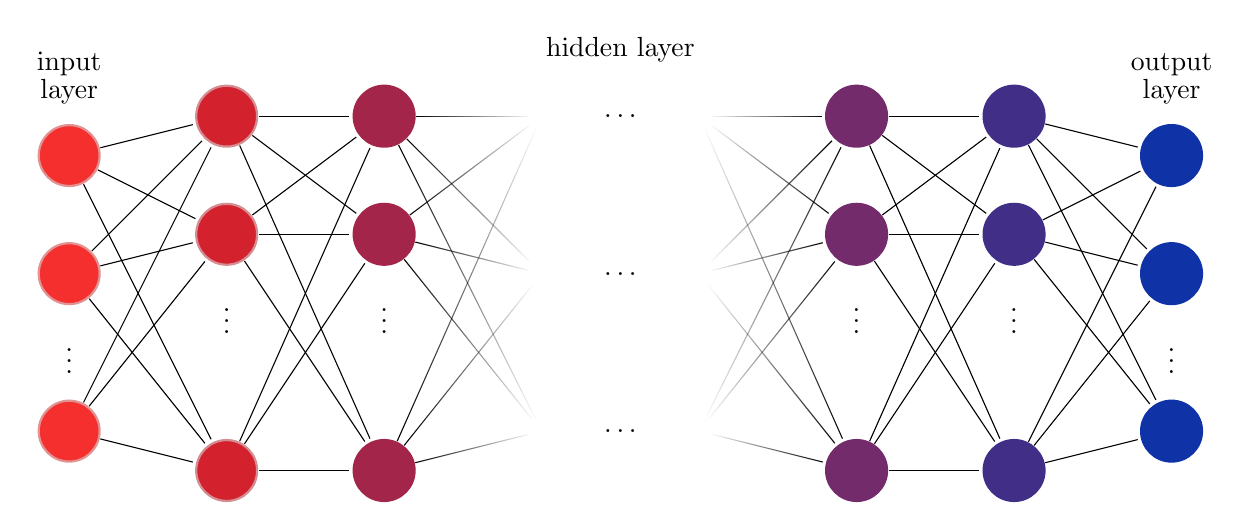
\begin{tikzpicture}[shorten >=1pt]
		\node[node in](x0) at (0,3.5){};
		\node[node in](x1) at (0,2){};
		\node at (0,1){\vdots};
		\node[node in](xd) at (0,0){};
 
		\node[hidden1](h10) at (2,4){};
		\node[hidden1](h11) at (2,2.5){};
		\node at (2,1.5){\vdots};
		\node[hidden1](h1m) at (2,-0.5){};

  		\node[hidden2](h20) at (4,4){};
		\node[hidden2](h21) at (4,2.5){};
		\node at (4,1.5){\vdots};
		\node[hidden2](h2m) at (4,-0.5){};
 
		\node(h32) at (6,0){};
		\node(h31) at (6,2){};
		\node(h30) at (6,4){};
		
		\node(d3) at (7,0){$\ldots$};
		\node(d2) at (7,2){$\ldots$};
		\node(d1) at (7,4){$\ldots$};

  		\node(hL12) at (8,0){};
		\node(hL11) at (8,2){};
		\node(hL10) at (8,4){};
  
   		\node[hidden3](hL20) at (10,4){};
		\node[hidden3](hL21) at (10,2.5){};
		\node at (10,1.5){\vdots};
		\node[hidden3](hL2m) at (10,-0.5){};
  
		
		\node[hidden4](hL30) at (12,4){};
		\node[hidden4](hL31) at (12,2.5){};
		\node at (12,1.5){\vdots};
		\node[hidden4](hL3m) at (12,-0.5){};
 
		\node[node out](y1) at (14,3.5){};
		\node[node out](y2) at (14,2){};
		\node at (14,1){\vdots};	
		\node[node out](yc) at (14,0){};
%Input layer to first hidden		
        \draw (x0) -- (h10);
		\draw (x0) -- (h11);
		\draw (x0) -- (h1m);
        
        \draw (x1) -- (h10);
		\draw (x1) -- (h11);
		\draw (x1) -- (h1m);
 
        \draw (xd) -- (h10);
		\draw (xd) -- (h11);
		\draw (xd) -- (h1m);
% first hidden to second hidden
        \draw (h10) -- (h20);
		\draw (h10) -- (h21);
		\draw (h10) -- (h2m);
        
        \draw (h11) -- (h20);
		\draw (h11) -- (h21);
		\draw (h11) -- (h2m);
 
        \draw (h1m) -- (h20);
		\draw (h1m) -- (h21);
		\draw (h1m) -- (h2m);
% second hidden to dissaper

       \draw[path fading=east] (h20) -- (h30);
		\draw[path fading=east] (h20) -- (h31);
		\draw[path fading=east] (h20) -- (h32);
		
	\draw[path fading=east] (h21) -- (h30);
		\draw[path fading=east] (h21) -- (h31);
		\draw[path fading=east] (h21) -- (h32);
		
	\draw[path fading=east] (h2m) -- (h30);
		\draw[path fading=east] (h2m) -- (h31);
		\draw[path fading=east] (h2m) -- (h32);

%dissaper to hidden L0i
		\draw[path fading=west] (hL10) -- (hL20);
		\draw[path fading=west] (hL11) -- (hL20);
		\draw[path fading=west] (hL12) -- (hL20);
		
		\draw[path fading=west] (hL10) -- (hL21);
		\draw[path fading=west] (hL11) -- (hL21);
		\draw[path fading=west] (hL12) -- (hL21);
		
		\draw[path fading=west] (hL10) -- (hL2m);
		\draw[path fading=west] (hL11) -- (hL2m);
		\draw[path fading=west] (hL12) -- (hL2m);
  
%        \draw (hL10) -- (hL20);
%            \draw (hL10) -- (hL21);
%            \draw (hL10) -- (hL2m);

%        \draw (hL11) -- (hL20);
%            \draw (hL11) -- (hL21);
%           \draw (hL11) -- (hL2m);

%        \draw (hL12) -- (hL20);
%            \draw (hL12) -- (hL21);
%            \draw (hL12) -- (hL2m);
            
% hidden L2m to L3m
        \draw (hL20) -- (hL30);
            \draw (hL20) -- (hL31);
            \draw (hL20) -- (hL3m);

        \draw (hL21) -- (hL30);
            \draw (hL21) -- (hL31);
            \draw (hL21) -- (hL3m);

        \draw (hL2m) -- (hL30);
            \draw (hL2m) -- (hL31);
            \draw (hL2m) -- (hL3m);

% hidden layer to output
		\draw (hL30) -- (y1);
		\draw (hL30) -- (yc);
		\draw (hL30) -- (y2);
 
		\draw (hL31) -- (y1);
		\draw (hL31) -- (yc);
		\draw (hL31) -- (y2);
 
		\draw (hL3m) -- (y1);
		\draw (hL3m) -- (y2);
		\draw (hL3m) -- (yc);
 

        \node[above=1,align=center] at (0,4) {input\\[-0.2em]layer};
        \node[above=2,align=center] at (7,4.5) {hidden layer};
        \node[above=1,align=center] at (14,4) {output\\[-0.2em]layer};  		
	\end{tikzpicture}
	\label{fig:multilayer-perceptron}
\end{figure}
 
\end{document}
